\newpage

\section{Word Embeddings}

\epigraph{
    Nets are for fish; once you get the fish you can forget the net.\\
    Words are for meaning; once you get the meaning you can forget the words.
}{Zhuangzi}
\newpage

\subsection{Dalla semantica alla rappresentazione vettoriale}
\label{sec:semantics_to_vectors}

Questo capitolo introduce il concetto di \textbf{embedding testuale}: una rappresentazione matematica che mappa simboli linguistici discreti (parole, token) in vettori continui capaci di catturare relazioni semantiche. Gli embeddings costituiscono il ponte tra il linguaggio naturale e l'elaborazione computazionale, permettendo alle macchine di manipolare il significato anziché limitarsi a confrontare stringhe di caratteri.
Come vedremo, la capacità di rappresentare efficacemente il significato linguistico in forma vettoriale è fondamentale per il lavoro sviluppato in questa tesi: gli sparse autoencoders (Capitolo~\ref{sec:autoencoders}) verranno applicati proprio a questi embeddings densi per estrarne strutture interpretabili. Prima di arrivare a tale applicazione, è necessario comprendere come si costruiscono gli embeddings, quali proprietà possiedono e come si sono evoluti dai modelli statici a quelli contestuali.

\subsubsection{Simboli e significati}
\label{subsubsec:symbols_meanings}
Il punto di partenza per comprendere gli \textit{embeddings} risiede nella distinzione tra \textbf{significante} e \textbf{significato}. In linguistica, il significante è la forma fisica del segno (il suono della parola o la stringa di caratteri ``mela''), mentre il significato è il concetto mentale a cui esso rimanda. Le macchine operano nativamente nel dominio dei significanti: esse manipolano simboli discreti che, per loro natura, sono arbitrari. Non vi è nulla nella stringa ``cane'' che richiami le proprietà biologiche dell'animale. 
La sfida dell'Intelligenza Artificiale è costruire una relazione, o funzione di mapping, che proietti l'insieme dei simboli in uno spazio semantico dove i concetti sono rappresentati numericamente.
\begin{figure}[htbp]
\centering
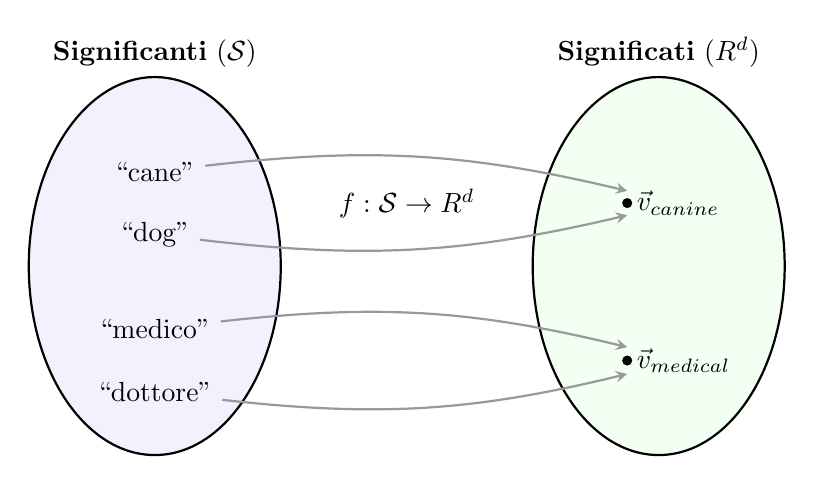
\begin{tikzpicture}[scale=0.8]
    % Insieme dei Significanti (Simboli)
    \draw[thick, fill=blue!5] (-4,0) ellipse (2cm and 3cm);
    \node[anchor=south] at (-4,3) {\textbf{Significanti} ($\mathcal{S}$)};
    \node (s1) at (-4,1.5) {``cane''};
    \node (s2) at (-4,0.5) {``dog''};
    \node (s3) at (-4,-1) {``medico''};
    \node (s4) at (-4,-2) {``dottore''};

    % Insieme dei Significati (Spazio Semantico)
    \draw[thick, fill=green!5] (4,0) ellipse (2cm and 3cm);
    \node[anchor=south] at (4,3) {\textbf{Significati} ($\mathbb{R}^d$)};
    
    % Punti nello spazio semantico
    \filldraw (3.5,1) circle (2pt) node[anchor=west] (v1) {$\vec{v}_{\text{canine}}$};
    \filldraw (3.5,-1.5) circle (2pt) node[anchor=west] (v2) {$\vec{v}_{\text{medical}}$};

    % Frecce di Mapping
    \draw[->, >=stealth, thick, gray!80] (s1) to [bend left=10] (v1);
    \draw[->, >=stealth, thick, gray!80] (s2) to [bend right=10] (v1);
    \draw[->, >=stealth, thick, gray!80] (s3) to [bend left=10] (v2);
    \draw[->, >=stealth, thick, gray!80] (s4) to [bend right=10] (v2);

    \node at (0,1) {$f: \mathcal{S} \to \mathbb{R}^d$};

\end{tikzpicture}
\caption{Rappresentazione del mapping tra lo spazio discreto dei simboli (Significanti) e lo spazio continuo dei vettori (Significati). L'obiettivo è apprendere una funzione $f$ tale che simboli diversi con significati simili vengano proiettati in vettori vicini nello spazio matematico.}
\label{fig:signifier_signified_mapping}
\end{figure}
Apprendere questa relazione è la \textit{conditio sine qua non} per permettere alle macchine di manipolare i simboli non solo come sequenze di bit, ma come entità portatrici di senso. Senza questo passaggio, il ragionamento logico e la coerenza semantica rimarrebbero preclusi.
\subsubsection{Gli assi del linguaggio}
\label{subsubsec:linguistic_axes}
\begin{figure}[h!]
    \centering
    \includegraphics[width=0.5\textwidth]{pictures/cap3/Ferdinand_de_Saussure_by_Jullien.png}
    \caption{Ferdinand de Saussure, fondatore della linguistica strutturale e teorico dei rapporti sintagmatici e associativi (paradigmatici) del linguaggio \cite{saussure_wikipedia_image}.}
    \label{fig:saussure}
\end{figure}
Per addestrare modelli capaci di catturare i significati dai significanti, li si pone nella condizione di analizzare enormi corpora di testo attraverso le due dimensioni fondamentali lungo le quali si articola ogni lingua: gli \textbf{assi saussuriani}.
\begin{figure}[htbp]
    \centering
    \begin{tikzpicture}[
        >=Stealth, 
        node distance=1.3cm,
        % Stile per la parola centrale (Pivot)
        target/.style={
            draw=black!80, 
            thick, 
            fill=yellow!10, 
            rounded corners=3pt, 
            inner sep=8pt, % Più spazio dentro il box
            font=\Large\bfseries
        },
        % Stile per l'asse orizzontale (Sintagma)
        syntagma/.style={
            font=\large, 
            text=black!90, 
            fill=white, % Fondamentale: copre la linea
            inner sep=3pt, % Margine bianco attorno alla parola per pulire la linea
            anchor=center
        },
        % Stile per l'asse verticale (Paradigma)
        paradigm/.style={
            font=\small\itshape, 
            text=black!60,
            fill=white, % Anche qui copriamo la linea verticale
            inner sep=2pt
        },
        % Stile per le etichette degli assi (Titoli)
        axislabel/.style={
            font=\sffamily\bfseries, 
            align=center
        },
        % Stile per le domande (piccolo e grigio)
        question/.style={
            font=\scriptsize\itshape, 
            text=black!60, 
            align=center
        }
    ]

        % --- ASSI ---
        % Allunghiamo leggermente le linee per dare respiro
        \draw[->, thick, blue!40!black!50] (-4.8, 0) -- (7.5, 0); 
        \draw[->, thick, red!40!black!50] (0, -3.8) -- (0, 4.8);

        % --- NODO CENTRALE ---
        \node[target] (center) at (0,0) {mangia};

        % --- PAROLE SINTAGMA (Orizzontale) ---
        % Posizionamento manuale per precisione
        \node[syntagma] at (-3.5, 0) {Il};
        \node[syntagma] at (-2.0, 0) {gatto};
        \node[syntagma] at (2.0, 0) {la};
        \node[syntagma] at (3.5, 0) {mela};

        % --- PAROLE PARADIGMA (Verticale) ---
        \node[paradigm] at (0, 1.4) {osserva};
        \node[paradigm] at (0, 2.2) {rincorre};
        \node[paradigm] at (0, 3.0) {annusa};
        
        \node[paradigm] at (0, -1.4) {divora};
        \node[paradigm] at (0, -2.2) {gusta};

        % --- ETICHETTE E DOMANDE ---
        
        % Asse Orizzontale
        % yshift=-0.2cm sposta il titolo un po' sotto la linea
        \node[axislabel, text=blue!40!black, anchor=north east] at (7.5, -0.2) {Asse Sintagmatico};
        % yshift negativo ulteriore per la domanda
        \node[question, anchor=north east] at (7.5, -0.7) {«Quale parola segue?»\\(Combinazione)};

        % Asse Verticale
        % yshift=0.2cm sposta il titolo sopra la punta
        \node[axislabel, text=red!40!black, anchor=south] at (0, 4.9) {Asse Paradigmatico};
        % Ancora più su per la domanda
        \node[question, anchor=south] at (0, 5.4) {«Cosa potrei mettere al posto di...?»\\(Selezione)};

    \end{tikzpicture}
    \caption{Rappresentazione degli assi del linguaggio. L'asse orizzontale mostra la sequenza lineare (sintagma), quello verticale le alternative possibili (paradigma).}
    \label{fig:linguistic_axes_final}
\end{figure}
L'\textbf{asse sintagmatico} riguarda la \textbf{combinazione}: risponde alla domanda \textit{«Quale parola segue?»} e governa la creazione di catene lineari (frasi). Al contrario, l'\textbf{asse paradigmatico} riguarda la \textbf{selezione}: risponde alla domanda \textit{«Cosa potrei mettere al posto di questa parola?»}. 
Gli algoritmi di embedding estraggono valore proprio all'intersezione di questi assi: analizzano le catene \textbf{sintagmatiche} osservabili nel testo per ricostruire lo spazio \textbf{paradigmatico} delle somiglianze. In fase di addestramento, il modello valuta quali termini siano intercambiabili in un dato contesto, mentre in fase di generazione opera sulla catena sintagmatica costruendo una sequenza coerente. È questa danza tra selezione e combinazione che permette l'emergere della coerenza semantica nei modelli moderni.

\subsubsection{L'ipotesi distribuzionale}
\label{subsubsec:distributional_hypothesis}

Per costruire queste relazioni di significato è necessario partire da un'ipotesi fondamentale. Supponiamo di non conoscere il significato della parola \textit{ongchoi}, ma di incontrarla nei seguenti contesti:

\begin{enumerate}
    \item \textit{L'ongchoi è deliziosa saltata con aglio.}
    \item \textit{L'ongchoi è ottima servita con riso.}
    \item \textit{...foglie di ongchoi con salse salate...}
\end{enumerate}

Ora immaginiamo di aver già visto molte di queste parole-contesto in altri esempi, come:

\begin{enumerate}
    \item \textit{...gli spinaci saltati con aglio serviti sul riso...}
    \item \textit{...le coste, con i loro gambi e foglie, sono molto gustose...}
    \item \textit{...il cavolo riccio e altre verdure a foglia dal sapore salato...}
\end{enumerate}

Il fatto che \textit{ongchoi} compaia insieme a parole come \textit{riso}, \textit{aglio}, \textit{deliziosa} e \textit{salata}, proprio come \textit{spinaci}, \textit{coste} o \textit{cavolo riccio}, suggerisce che l'ongchoi sia una verdura a foglia simile a queste altre verdure. Questo è il principio dell'ipotesi distribuzionale per il quale parole semanticamente simili tendono a comparire in contesti simili.

\begin{notebox}
\textbf{Ipotesi Distribuzionale}\\
Si definisce ipotesi distribuzionale quella ipotesi per la quale parole simili compaiono in contesti simili. 
\end{notebox}

Tale ipotesi suggerisce che il significato delle parole venga appreso sulla base del contesto in cui queste appaiono. Se questa intuizione viene seguita, allora diventa possibile assegnare rappresentazioni numeriche alle parole sulla base della loro occorrenza in contesti specifici. Prima di arrivare però a capire come costruire gli embeddings è necessario introdurre una ulteriore intuizione attribuita ad Osgood nel 1957.

\subsubsection{Ipotesi di Osgood: il significato come vettore}
\label{subsubsec:osgood_hypothesis}

Un contributo fondamentale alla rappresentazione del significato proviene dal lavoro di Osgood \parencite{Osgood1957Measurement}, che studiò la componente affettiva delle parole. Osgood mostrò che i giudizi emotivi associati a una parola possono essere descritti lungo tre dimensioni principali:

\begin{enumerate}
    \item \textbf{Valenza}: quanto la parola è percepita come positiva o negativa.
    \item \textbf{Arousal}: quanto la parola induce attivazione emotiva.
    \item \textbf{Dominanza}: quanto la parola implica controllo o sottomissione.
\end{enumerate}

Ogni parola può quindi essere rappresentata come una tripla di valori numerici che ne definiscono la posizione in questo spazio tridimensionale. Ad esempio:
\[
\textit{heartbreak} \rightarrow [2.5,\ 5.7,\ 3.6]
\]

L'intuizione rivoluzionaria di Osgood è la seguente:

\begin{notebox}
\textbf{Ipotesi di Osgood}\\
Il significato di una parola può essere rappresentato come un vettore in uno spazio semantico.
\end{notebox}

Questa idea è stata la prima ad anticipare direttamente i moderni modelli di \textit{word embeddings}, in cui ogni parola è descritta come un punto in uno spazio multidimensionale corrispondente a un significato. Mentre Osgood lavorava con tre dimensioni interpretabili psicologicamente, i modelli computazionali moderni utilizzano centinaia o migliaia di dimensioni apprese automaticamente dai dati, catturando relazioni semantiche complesse che vanno ben oltre la dimensione affettiva.

\subsubsection{Verso i word embeddings}
\label{subsubsec:towards_embeddings}
L'unione dell'ipotesi distribuzionale e dell'ipotesi di Osgood ha aperto la strada agli embeddings come modello fondamentale per la rappresentazione computazionale del significato. Da un lato, l'ipotesi distribuzionale fornisce il principio secondo cui il significato delle parole può essere inferito dai contesti in cui esse compaiono; dall'altro, l'ipotesi di Osgood suggerisce che tale significato possa essere rappresentato come un vettore numerico in uno spazio semantico.
Nelle sezioni successive introdurremo le principali famiglie di embeddings, partendo dai modelli basati su conteggi (count-based) fino ai moderni embeddings contestuali prodotti da architetture Transformer. Per orientare il lettore, è utile chiarire fin da subito le principali tipologie di embeddings che verranno introdotte nel seguito.
In base alla natura della rappresentazione prodotta, è possibile distinguere due grandi famiglie: embeddings \textbf{statici} ed embeddings \textbf{dinamici}.
\begin{figure}[htbp]
\centering
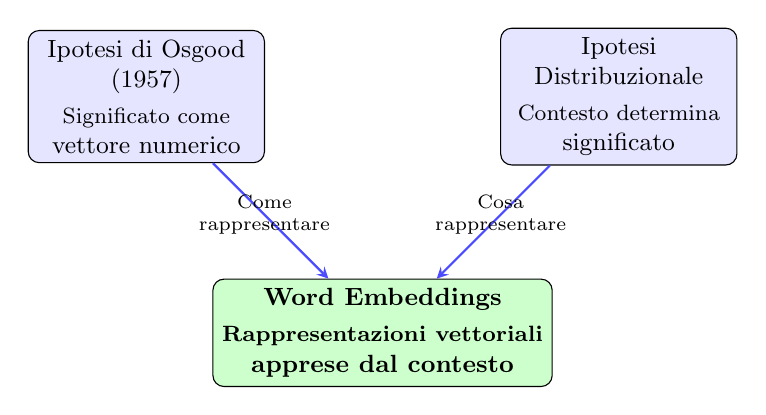
\begin{tikzpicture}[
    node distance=2cm,
    box/.style={draw, rectangle, rounded corners, minimum width=3cm, minimum height=1cm, align=center, font=\small, fill=blue!10},
    result/.style={draw, rectangle, rounded corners, minimum width=4cm, minimum height=1.2cm, align=center, font=\small\bfseries, fill=green!20},
    arrow/.style={->, >=stealth, thick}
]
    % Ipotesi di partenza
    \node[box] (osgood) at (-3, 2) {Ipotesi di Osgood\\(1957)\\[0.2em]\footnotesize Significato come\\vettore numerico};
    
    \node[box] (distributional) at (3, 2) {Ipotesi\\Distribuzionale\\[0.2em]\footnotesize Contesto determina\\significato};
    
    % Risultato
    \node[result] (embeddings) at (0, -1) {Word Embeddings\\[0.2em]\footnotesize Rappresentazioni vettoriali\\apprese dal contesto};
    
    % Frecce convergenti
    \draw[arrow, blue!70] (osgood) -- (embeddings);
    \draw[arrow, blue!70] (distributional) -- (embeddings);
    
    % Etichette sulle frecce
    \node[font=\scriptsize, text width=2cm, align=center] at (-1.5, 0.5) {Come\\rappresentare};
    \node[font=\scriptsize, text width=2cm, align=center] at (1.5, 0.5) {Cosa\\rappresentare};

\end{tikzpicture}
\caption{Convergenza delle due ipotesi fondamentali negli embeddings moderni. L'ipotesi di Osgood fornisce il \emph{formato} della rappresentazione (vettori numerici), mentre l'ipotesi distribuzionale indica \emph{cosa} deve essere catturato (relazioni contestuali tra parole).}
\label{fig:convergenza_ipotesi}
\end{figure}
\begin{notebox}
\textbf{Embeddings statici}\\
Si definisce statico un embedding in cui ogni parola del vocabolario è associata a un unico vettore pre-computato. Tale rappresentazione rimane invariata a prescindere dal contesto specifico in cui la parola appare.
\end{notebox}
Negli embeddings statici, a ciascun tipo di parola del vocabolario è associato un unico vettore, indipendente dal contesto in cui la parola appare. Questa categoria include sia gli embeddings distribuzionali basati su conteggi, come le matrici termine--documento e termine--termine eventualmente ridotte tramite SVD, sia gli embeddings predittivi appresi mediante modelli neurali, come Word2Vec.
\begin{notebox}
\textbf{Embeddings dinamici (Contestuali)}\\
Si definisce dinamico un embedding in cui la rappresentazione vettoriale di una parola viene computata in modo dipendente dal contesto, come funzione dell'intera sequenza di input. La stessa parola riceve quindi vettori diversi a seconda del contesto semantico e sintattico in cui compare.\end{notebox}
Gli embeddings dinamici, o contestuali, producono invece una rappresentazione dipendente dal contesto: la stessa parola può essere associata a vettori diversi a seconda della frase in cui compare. Tali rappresentazioni sono generate da modelli di linguaggio neurali profondi, a partire da architetture ricorrenti fino ai moderni modelli Transformer, come BERT.
\begin{figure}[htbp]
\centering
\begin{forest}
  for tree={
    draw,
    rounded corners,
    fill=blue!5,
    align=center,
    font=\small,
    edge={->, thick},
    l sep=1.2cm,    
    s sep=0.5cm,
    inner sep=6pt
  }
  [\textbf{Embeddings}
    [\textbf{Statici}
      [{\textbf{Count-based}\\(Term-Doc, Term-Term)}]
      [{\textbf{Predittivi neurali}\\(Word2Vec, GloVe)}]
    ]
    [\textbf{Dinamici}
      [{\textbf{Modelli neurali profondi}\\(ELMo, BERT, GPT)}]
    ]
  ]
\end{forest}
\caption{Classificazione delle principali tipologie di embeddings trattate nel capitolo.}
\label{fig:classificazione_embeddings}
\end{figure}
La Figura~\ref{fig:classificazione_embeddings} riassume questa tassonomia. Nelle sezioni successive analizzeremo in dettaglio ciascuna di queste famiglie, comprendendo come si costruiscono, quali proprietà possiedono e quali limiti presentano. Questo percorso ci condurrà fino agli embeddings densi prodotti da modelli come BERT, che costituiscono l'input degli Sparse Autoencoders discussi nel Capitolo~\ref{sec:04_disentangling_dense_embeddings_with_sparse_autoencoders}.
\subsection{Embeddings statici}
\label{sec:static_embeddings}
In questa sezione introduciamo gli embeddings statici, rappresentazioni in cui ogni parola del vocabolario è associata a un unico vettore fisso, indipendente dal contesto in cui compare. Distingueremo tra due approcci fondamentali: i metodi \textbf{count-based}, che costruiscono rappresentazioni a partire da statistiche di co-occorrenza, e i metodi \textbf{predittivi}, che apprendono embeddings tramite reti neurali addestrate a predire parole in contesto.
\subsubsection{Embeddings count-based}
\label{subsubsec:count_based}
Il modo più semplice per costruire embeddings vettoriali delle parole è basato sulla \textbf{matrice di co-occorrenza}, una struttura che codifica quante volte determinati elementi linguistici compaiono insieme all'interno di un corpus. Esistono diverse varianti di matrici di co-occorrenza; in questa sezione ne introduciamo due fondamentali: la \emph{term-document matrix} e la \emph{term-term matrix}.
\paragraph{Matrice termine-documento.}
In una matrice termine-documento ogni riga rappresenta una parola del vocabolario e ogni colonna rappresenta un documento appartenente a una collezione di testi. Ogni cella della matrice contiene il numero di volte in cui la parola associata alla riga compare nel documento associato alla colonna. Un esempio di term-document matrix è riportato nella Tabella~\ref{tab:term_document_shakespeare}, che mostra le occorrenze di quattro parole in quattro opere di Shakespeare.

\begin{table}[h!]
\centering
\begin{tabular}{lcccc}
\hline
 & \textbf{As You Like It} & \textbf{Twelfth Night} & \textbf{Julius Caesar} & \textbf{Henry V} \\
\hline
battle & 1   & 0  & 7  & 13 \\
good   & 114 & 80 & 62 & 89 \\
fool   & 36  & 58 & 1  & 4  \\
wit    & 20  & 15 & 2  & 3  \\
\hline
\end{tabular}
\caption{Term-document matrix per quattro parole in quattro opere di Shakespeare. Ogni cella contiene il numero di occorrenze della parola (riga) nel documento (colonna).}
\label{tab:term_document_shakespeare}
\end{table}
Questa matrice può essere interpretata in due modi distinti ma complementari. Se si considerano le \textbf{colonne} della matrice, ciascun documento è rappresentato come un vettore in uno spazio di dimensione $|V|$, dove $|V|$ è la dimensione del vocabolario. Tale rappresentazione costituisce il fondamento del \emph{vector space model} per il recupero dell'informazione. 
Alternativamente, se si considerano le \textbf{righe} della matrice, ogni parola può essere interpretata come un vettore in uno spazio di dimensione pari al numero di documenti.
\begin{notebox}
\textbf{Interpretazione delle righe della matrice termine-documento}\\
Due parole risultano simili se presentano distribuzioni simili sui documenti, ovvero se tendono a comparire negli stessi testi con frequenze comparabili.
\end{notebox}
La term-document matrix fornisce quindi una prima, semplice forma di \emph{embedding distribuzionale} delle parole, in cui il significato emerge dalla loro distribuzione nei documenti del corpus.
\paragraph{Matrice termine-termine.}
Un'alternativa alla matrice termine--documento per la rappresentazione distribuzionale delle parole è la matrice termine-termine, detta anche \emph{word--word matrix} o \emph{term--context matrix}. In questo caso, le colonne della matrice non sono più etichettate da documenti, bensì da parole del vocabolario. La matrice ha quindi dimensionalità $|V| \times |V|$, dove $|V|$ indica la dimensione del vocabolario.
In una matrice termine-termine, ogni riga rappresenta una \textbf{parola target} e ogni colonna rappresenta una \textbf{parola di contesto}. Ciascuna cella contiene il numero di volte in cui la parola di contesto compare nel contesto della parola target all'interno di un corpus di addestramento. Il concetto di \emph{contesto} viene tipicamente definito tramite una \textbf{finestra scorrevole} attorno alla parola target. Ad esempio, fissata una finestra di ampiezza $\pm k$, una parola è considerata di contesto se compare entro $k$ posizioni a sinistra o a destra della parola target nel testo.
La Tabella~\ref{tab:term_term_wikipedia} riporta un estratto reale di una matrice termine--termine calcolata sul corpus Wikipedia.
\begin{table}[h!]
\centering
\begin{tabular}{lcccccc}
\hline
\textbf{Parola} & \textbf{aardvark} & \textbf{computer} & \textbf{data} & \textbf{result} & \textbf{pie} & \textbf{sugar} \\
\hline
cherry       & 0 & 2    & 8    & 9    & 442 & 25 \\
strawberry   & 0 & 0    & 0    & 1    & 60  & 19 \\
digital      & 0 & 1670 & 1683 & 85   & 5   & 4  \\
information  & 0 & 3325 & 3982 & 378  & 5   & 13 \\
\hline
\end{tabular}
\caption{Estratto di una matrice termine--termine calcolata sul corpus Wikipedia. Ogni cella contiene il numero di co-occorrenze tra la parola target (riga) e la parola di contesto (colonna) all'interno di una finestra di contesto locale.}
\label{tab:term_term_wikipedia}
\end{table}
In questa rappresentazione, ogni parola è associata a un vettore in uno spazio di dimensione $|V|$, in cui ciascuna dimensione corrisponde a una parola di contesto. Parole semanticamente simili tendono ad avere vettori simili, poiché compaiono in contesti linguistici analoghi.
\begin{notebox}
\textbf{Interpretazione della matrice termine--termine}\\
Due parole risultano semanticamente simili se presentano vettori di co-occorrenza simili, ovvero se tendono a comparire negli stessi contesti linguistici, anche nel caso in cui non compaiano mai direttamente insieme.
\end{notebox}
Data $|V|$ la dimensione del vocabolario, tale matrice ha una dimensionalità $|V| \times |V|$. Si hanno tuttavia due problemi:
\begin{enumerate}
    \item Dal momento che ogni parola co-occorrerà solo con pochissime altre, \textit{la dimensionalità della matrice è enorme}.
    \item La maggior parte delle celle è nulla, e quindi \textit{i vettori sono estremamente sparsi}.
\end{enumerate}
Per affrontare questi problemi esistono diverse strategie, tra cui la riduzione dimensionale tramite SVD e il passaggio a paradigmi predittivi come Word2Vec.
\paragraph{Riduzione dimensionale tramite SVD.}
Un metodo per la riduzione della dimensionalità è la Singular Value Decomposition applicata alla word--context matrix. Sia $M \in \mathbb{R}^{|V| \times |V|}$ la word--context matrix, eventualmente pesata tramite tf-idf. La decomposizione ai valori singolari consente di fattorizzare $M$ come prodotto di tre matrici:
\[
M = U \Sigma V^\top
\]
dove $U$ e $V$ sono matrici ortogonali e $\Sigma$ è una matrice diagonale contenente i valori singolari ordinati in modo decrescente. Per ottenere una rappresentazione a dimensionalità ridotta, si considera una versione troncata della decomposizione, mantenendo solo i primi $k$ valori singolari:
\[
M \approx U_k \Sigma_k V_k^\top
\]
con $k \ll |V|$. Le righe della matrice $U_k \Sigma_k$ costituiscono una rappresentazione densa delle parole target in uno spazio latente di dimensione $k$. In questo nuovo spazio, ogni parola è descritta da un vettore a dimensionalità ridotta, in cui le correlazioni semantiche risultano più evidenti rispetto alla rappresentazione originale sparsa.
\paragraph{Cosine similarity.}
Una volta ottenuti vettori di embedding (sia da matrici di co-occorrenza sia da riduzione dimensionale), serve una metrica per quantificare la similarità semantica tra parole. La \textbf{cosine similarity} è una misura di similarità tra vettori che valuta il coseno dell'angolo compreso tra essi nello spazio vettoriale. Data la sua indipendenza dalla lunghezza dei vettori, risulta particolarmente adatta a confrontare vettori di frequenze o di pesi.
Dati due vettori $u$ e $v$, la similarità coseno è definita come:
\begin{equation}
\text{cosine\_sim}(u, v) = 
\frac{u \cdot v}{\|u\| \, \|v\|}
= \frac{\sum_i u_i v_i}{\sqrt{\sum_i u_i^2} \, \sqrt{\sum_i v_i^2}}.
\end{equation}
Il valore risultante è compreso tra $-1$ e $1$: $1$ indica massima similarità (stessa direzione), $0$ indica ortogonalità (nessuna similarità), e valori negativi indicano direzioni opposte. Nelle applicazioni di NLP la cosine similarity è spesso preferita alla distanza Euclidea, perché ci interessa confrontare il \textit{pattern} delle co-occorrenze piuttosto che le loro magnitudini assolute.
\subsubsection{Word2Vec: un approccio predittivo}
\label{subsubsec:word2vec}
\begin{figure}[htbp]
\centering
\begin{tikzpicture}[
    node distance=0.8cm,
    theory/.style={draw, ellipse, minimum width=2.5cm, minimum height=1cm, align=center, font=\footnotesize, fill=blue!10},
    impl/.style={draw, rectangle, rounded corners, minimum width=2.5cm, minimum height=0.8cm, align=center, font=\footnotesize, fill=green!15}
]
    % Colonna sinistra: Osgood
    \node[theory] (osg_theory) at (-3, 3.5) {
        \textbf{Osgood}\\
        {\scriptsize Significato $\to$ vettore}
    };
    
    \node[impl] (osg_vectors) at (-3, 2) {
        Matrici $W$, $C$\\
        $\mathbf{w}, \mathbf{c} \in \mathbb{R}^d$
    };
    
    \node[impl] (osg_sim) at (-3, 0.8) {
        Similarità:\\
        $\mathbf{w} \cdot \mathbf{c}$
    };
    
    % Colonna destra: Distribuzionale
    \node[theory] (dist_theory) at (3, 3.5) {
        \textbf{Distribuzionale}\\
        {\scriptsize Contesto $\to$ significato}
    };
    
    \node[impl] (dist_window) at (3, 2) {
        Finestra $\pm k$\\
        Contesto locale
    };
    
    \node[impl] (dist_cooc) at (3, 0.8) {
        Co-occorrenze\\
        $P(c \mid w)$
    };
    
    % Frecce
    \draw[->, thick, blue!60] (osg_theory) -- (osg_vectors);
    \draw[->, thick, blue!60] (osg_vectors) -- (osg_sim);
    \draw[->, thick, blue!60] (dist_theory) -- (dist_window);
    \draw[->, thick, blue!60] (dist_window) -- (dist_cooc);
    
    % Word2Vec al centro in basso
    \node[draw, rectangle, rounded corners, fill=orange!20, minimum width=7cm, minimum height=1cm, align=center, font=\small\bfseries] (w2v) at (0, -0.8) {
        Word2Vec\\
        {\footnotesize $\max \sum \log \sigma(\mathbf{w} \cdot \mathbf{c})$ per $(w,c)$ in finestra $k$}
    };
    
    \draw[->, thick, gray] (osg_sim) -- (w2v);
    \draw[->, thick, gray] (dist_cooc) -- (w2v);

\end{tikzpicture}
\caption{Word2Vec come fusione tra teoria e implementazione. A sinistra, l'ipotesi di Osgood si traduce nella scelta di vettori continui e nel prodotto scalare come misura di similarità. A destra, l'ipotesi distribuzionale si concretizza nella finestra di contesto e nella modellazione di co-occorrenze. Word2Vec unifica elegantemente queste due linee, apprendendo vettori che massimizzano la predizione di co-occorrenze locali.}
\label{fig:word2vec_teoria_implementazione}
\end{figure}
Sebbene i metodi basati su conteggi e la riduzione dimensionale tramite SVD permettano di ottenere rappresentazioni semanticamente dense, essi presentano limiti strutturali non trascurabili. Il calcolo della decomposizione ai valori singolari su matrici di co-occorrenza è computazionalmente oneroso, con una complessità che cresce sensibilmente rispetto alla dimensione del vocabolario, rendendo difficile la scalabilità su corpora massicci.
Per superare queste criticità, Mikolov et al. hanno introdotto \textit{Word2Vec} \parencite{mikolov2013efficientestimationwordrepresentations}, un framework basato su un paradigma radicalmente diverso: la \textbf{predizione}. Invece di riassumere statistiche globali, Word2Vec apprende gli embeddings processando il testo localmente. Lo spostamento di paradigma risiede nel fatto che, anziché contare le occorrenze totali, addestriamo un classificatore su un compito di \textbf{classificazione binaria}. Il modello deve rispondere alla domanda:
\begin{center}
\textit{``Data la parola target $w$ (es. \textit{albicocca}), qual è la probabilità che la parola candidata $c$ (es. \textit{marmellata}) compaia nel suo contesto?''}
\end{center}
In questo approccio, noto come \textbf{self-supervision}, il testo stesso fornisce le etichette: ogni parola $c$ che appare effettivamente vicino a $w$ nel corpus fornisce un esempio positivo (etichetta $1$), dovo per ``vicino" si intende dentor una finstra di contesto di $k$ parole. Al contrario, per addestrare il classificatore, il modello genera artificialmente degli esempi negativi campionando parole casuali dal vocabolario che non compaiono nel contesto di $w$ (etichetta $1$).
\paragraph{Il classificatore e la funzione sigmoide.}
L'intuizione alla base del classificatore è che due parole siano semanticamente vicine se i loro vettori di embedding sono simili. Per misurare questa affinità, utilizziamo il \textbf{prodotto scalare} tra il vettore della parola target $\mathbf{w}$ e il vettore della parola di contesto $\mathbf{c}$:
\[
\text{Similarity}(w,c) \approx \mathbf{w} \cdot \mathbf{c}
\]

Poiché il prodotto scalare può assumere qualsiasi valore reale, utilizziamo la funzione \textbf{sigmoide} $\sigma(x)$ per mappare il risultato in una probabilità compresa tra $0$ e $1$:
\begin{equation}
\sigma(x) = \frac{1}{1 + e^{-x}}
\end{equation}

Il modello stima quindi la probabilità che la coppia $(w, c)$ sia un esempio positivo ($+$) come:
\begin{equation}
P(+ \mid w, c) = \sigma(\mathbf{w} \cdot \mathbf{c}) = \frac{1}{1 + e^{-\mathbf{w} \cdot \mathbf{c}}}
\end{equation}

Nel caso generale, data una parola target $w$ e un'intera finestra di $L$ parole di contesto $c_{1:L}$, il modello assume che le parole nel contesto siano indipendenti tra loro. La probabilità complessiva è dunque data dal prodotto delle probabilità individuali:
\begin{equation}
\log P(+ \mid w, c_{1:L}) = \sum_{i=1}^L \log \sigma(\mathbf{w} \cdot \mathbf{c}_i)
\end{equation}

\paragraph{Perché due matrici? Il ruolo di $W$ e $C$.}
Una caratteristica distintiva di Word2Vec è il mantenimento di \textit{due rappresentazioni distinte} per ogni parola, organizzate in due matrici di pesi separate (Figura~\ref{fig:skipgram_structure}). Una matrice $W$ relativa alle parole target che contiene i vettori utilizzati quando la parola è il centro della finestra, e una matrice $C$ che contiene i vettori utilizzati quando la parola appare nel contesto di un'altra o viene estratta come esempio negativo.

\begin{figure}[h!]
    \centering
    \includegraphics[width=0.7\textwidth]{pictures/embeddings_w2vec.png}
    \caption{Lo skip-gram apprende in totale due insiemi di embedding, uno per i target ($W$) e uno per i contesti ($C$), per un totale di $2|V|$ vettori. L'addestramento mira a massimizzare la probabilità che parole vicine nel testo abbiano vettori simili.}
    \label{fig:skipgram_structure}
\end{figure}

Sdoppiando le matrici, il modello garantisce la \textit{stabilità dell'ottimizzazione}. Se usassimo un unico vettore $\mathbf{v}$, il modello cercherebbe di massimizzare il prodotto scalare $\mathbf{v} \cdot \mathbf{v}$ (auto-similarità), portando i valori a crescere all'infinito. Con due matrici, il modello apprende relazioni distribuzionali senza questo vincolo. Al termine, si utilizzano solitamente i vettori di $W$ o la media $W+C$.
\paragraph{Finestra di contesto e precisione semantica.}
L'ampiezza della finestra di contesto $k$ controlla quanta informazione sintagmatica il modello può sfruttare per inferire il paradigma semantico. All'aumentare di $k$, il modello osserva un contesto più ampio e cattura relazioni semantiche progressivamente più ricche.
\begin{itemize}
    \item \textit{Finestra stretta} ($k$ piccolo): il contesto è locale e cattura principalmente regolarità \textit{funzionali e sintattiche}. Gli embeddings risultanti tendono a raggruppare parole che svolgono ruoli grammaticali simili.
    \item \textit{Finestra ampia} ($k$ grande): il contesto include indizi più distanti, catturando affinità \textit{semantiche e tematiche}. Ad esempio, parole come \textit{ospedale} e \textit{medico} non sono intercambiabili sintatticamente, ma co-occorrono in ambienti discorsivi simili e risultano quindi vicine nello spazio vettoriale.
\end{itemize}
Questa relazione tra ampiezza della finestra e tipo di similarità catturata riflette direttamente il principio degli assi saussuriani: osservando porzioni più ampie della catena sintagmatica, il modello ricostruisce con maggiore precisione lo spazio paradigmatico delle sostituzioni semanticamente plausibili.
\paragraph{Geometria dell'analogia: il modello del parallelogramma.}
Quando lo spazio latente è coerente, non si limita a raggruppare parole simili: tende anche a codificare \textit{relazioni} come direzioni stabili. Questo si manifesta nel ragionamento analogico, spesso descritto tramite il cosiddetto modello del parallelogramma. 

\begin{notebox}
\textbf{Modello del parallelogramma}\\
Le relazioni semantiche possono essere codificate come differenze vettoriali approssimativamente costanti. Data l'analogia «$a$ sta ad $a^*$ come $b$ sta ad $b^*$» (es.\ \textit{uomo}:\textit{donna} = \textit{re}:\textit{regina}), il termine incognito $b^*$ è approssimabile come:
\[ b^* \approx b - a + a^* \]
\end{notebox}

\begin{figure}[htbp]
\centering
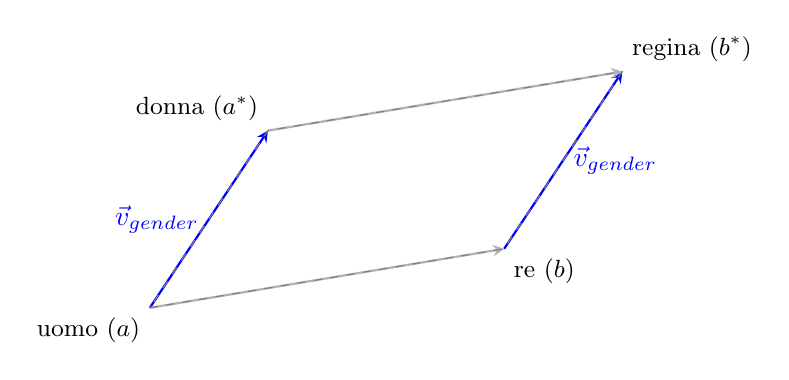
\begin{tikzpicture}[scale=1.5, >=stealth]
    \coordinate (man) at (0,0);
    \coordinate (woman) at (1,1.5);
    \coordinate (king) at (3,0.5);
    \coordinate (queen) at (4,2);

    \draw[->, thick, blue] (man) -- (woman) node[midway, left] {$\vec{v}_{gender}$};
    \draw[->, thick, blue] (king) -- (queen) node[midway, right] {$\vec{v}_{gender}$};
    \draw[->, thick, gray!60] (man) -- (king);
    \draw[->, thick, gray!60] (woman) -- (queen);

    \node[below left] at (man) {\small uomo ($a$)};
    \node[above left] at (woman) {\small donna ($a^*$)};
    \node[below right] at (king) {\small re ($b$)};
    \node[above right] at (queen) {\small regina ($b^*$)};

    \draw[dashed, gray] (man) -- (king) -- (queen) -- (woman) -- cycle;
\end{tikzpicture}
\caption{Rappresentazione geometrica del modello del parallelogramma nello spazio latente.}
\label{fig:parallelogramma}
\end{figure}

\subsubsection{Limiti degli embeddings statici}
\label{subsubsec:static_limits}
La logica ``più sintagma $\Rightarrow$ paradigma più preciso'' evidenzia però un limite intrinseco di Word2Vec: anche se durante l'addestramento sfrutta il contesto, il risultato finale è un \textbf{embedding statico}. Una volta appresi i vettori, ogni parola è associata a un'unica rappresentazione, indipendente dall'uso concreto in frase. Questo comporta almeno due criticità fondamentali:
\begin{enumerate}
    \item \textit{Polisemia:} una parola con più sensi (es.\ \textit{banco} come mobile o come istituzione finanziaria) viene compressa in un unico vettore che media usi diversi, riducendo la precisione semantica proprio dove il contesto dovrebbe aiutare.
    \item \textit{Contesto ``dimenticato'' in inferenza:} Word2Vec usa la finestra sintagmatica per \emph{apprendere} i vettori, ma in \textit{inferenza} l'embedding di una parola è recuperato come valore fisso dal dizionario del modello e non viene ricalcolato in funzione della frase specifica. Di conseguenza, la stessa parola mantiene lo stesso vettore anche in contesti diversi, e il contesto non può più agire da meccanismo di disambiguazione.
\end{enumerate}
\begin{notebox}
\textbf{Training vs inferenza}\\
Per \textbf{inferenza} si intende l'uso del modello \emph{dopo} l'addestramento: dati nuovi input, i parametri appresi $\theta$ restano fissi e il modello calcola solo le sue uscite. In Word2Vec, durante l'addestramento il contesto influenza l'apprendimento dei vettori; in inferenza, però, ogni parola ha un embedding fisso indipendente dal contesto in cui compare.
\end{notebox}
Se il significato di una parola dipende sistematicamente dalla ricchezza del sintagma che la circonda, allora la rappresentazione dovrebbe essere una \textbf{funzione del contesto}, non una costante. Questa osservazione motiva il passaggio agli \textbf{embeddings dinamici (contestuali)}: invece di limitarsi a una finestra fissa e a un vettore unico per parola, essi mirano a incorporare informazione proveniente dall'intera sequenza, generando un vettore diverso per ogni occorrenza. 
Per ottenere questo comportamento servono architetture in grado di modellare il linguaggio come flusso e memoria. Nella prossima sezione introdurremo brevemente le architetture ricorrenti e il meccanismo di attenzione, che preparano il terreno per i moderni Transformer e, in particolare, per BERT—il modello che produce gli embeddings densi su cui applicheremo gli Sparse Autoencoders nei capitoli successivi.




%%%%%%%%%%%%%%%%%%%%%%%%%%%%%%%%%%%%%%%%%%

\subsection{Embeddings dinamici (contestuali)}
\label{sec:dynamic_embeddings}

La sezione precedente ha mostrato come Word2Vec sfrutti il contesto sintagmatico durante l'addestramento per apprendere vettori semanticamente ricchi. Tuttavia, una volta completato il training, il risultato è un dizionario di rappresentazioni fisse: in fase di inferenza, l'embedding di una parola viene semplicemente recuperato da una tabella di lookup, indipendentemente dalle parole che la circondano nella frase concreta.
Questo limite diventa evidente nei casi di polisemia. La parola \textit{pesca}, ad esempio, può riferirsi a un frutto (\textit{``La pesca è matura''}) o a un'attività (\textit{``La pesca in questo lago è vietata''}). In un modello statico, entrambi gli usi vengono collassati in un unico punto dello spazio vettoriale—una sorta di ``media'' tra sensi incompatibili. Ma il principio sintagma-paradigma discusso nella Sezione~\ref{subsubsec:linguistic_axes} suggerisce l'opposto: il senso corretto non è una proprietà isolata del token, bensì emerge dall'interazione con il contesto in cui quel token è inserito.
Se un sintagma più ricco rende più preciso il paradigma, allora la rappresentazione di una parola dovrebbe essere una funzione del contesto, non una costante. Questo è esattamente ciò che gli embeddings dinamici (o contestuali) si propongono di fare: invece di associare un vettore a un \emph{tipo} lessicale (\textit{word type}), associano un vettore a ciascuna \emph{occorrenza} concreta (\textit{word token}), calcolandolo come funzione dell'intera sequenza in cui la parola appare.
\begin{notebox}
\textbf{Embedding dinamico (contestuale)}\\
Data una sequenza di token $x_1, \dots, x_n$, un embedding dinamico è una rappresentazione vettoriale $h_i$ per il token $x_i$ tale che
\[
h_i = f(x_i, x_{1:n}),
\]
dove $f$ è una funzione che integra informazione dall'intera sequenza. A differenza degli embeddings statici, $h_i$ dipende dal contesto: la stessa parola riceve vettori diversi in frasi diverse.
\end{notebox}
In pratica, queste rappresentazioni emergono dagli stati interni di modelli neurali che processano sequenze. Un embedding statico è un parametro appreso e poi fissato; un embedding dinamico è invece un'attivazione della rete calcolata in inferenza, che cambia al variare del contesto. Per questo motivo, la stessa parola può corrispondere a vettori diversi in frasi diverse: il modello integra informazione sintattica e semantica dalle parole circostanti, disambiguando il senso in modo implicito.
A questo punto la domanda diventa: come si costruisce una funzione $f$ capace di integrare contesto su sequenze lunghe senza perdere informazione? La storia recente delle architetture neurali per il linguaggio può essere letta come una sequenza di risposte progressive a questo problema. Nelle sezioni successive seguiremo questa evoluzione:
\begin{enumerate}
    \item Le RNN introducono memoria sequenziale, ma soffrono di \textit{vanishing gradient}.
    \item Le LSTM risolvono il vanishing gradient con gate di memoria, ma rimangono unidirezionali e sequenziali.
    \item La bidirezionalità permette di integrare contesto da entrambe le direzioni—ma per task che richiedono di \textit{trasformare} una sequenza in un'altra servono architetture diverse.
    \item L'Encoder-Decoder affronta i task sequence-to-sequence, ma introduce un collo di bottiglia informativo.
    \item Il meccanismo di attenzione supera il bottleneck, permettendo accesso diretto a tutta la sequenza sorgente—ma l'architettura rimane ricorrente.
    \item I Transformer eliminano la ricorrenza usando solo self-attention, rendendo il calcolo parallelizzabile e l'addestramento su larga scala finalmente fattibile.
    \item BERT sfrutta la self-attention bidirezionale con un nuovo obiettivo di pre-training—il \textit{masked language modeling}—producendo embeddings contestuali potenti ma opachi.
\end{enumerate}
Ogni architettura risolve un limite della precedente, introducendo al contempo nuove sfide. Questo percorso ci condurrà fino agli embeddings densi di BERT, la cui opacità motiva il lavoro della presente tesi: nel Capitolo~\ref{sec:04_disentangling_dense_embeddings_with_sparse_autoencoders} introdurremo gli Sparse Autoencoders come strumento per estrarre feature interpretabili da queste rappresentazioni.

%%%%%%%%%%%%%%%%%%%%%%%%%%%%%%%%%%%%


\subsubsection{RNN: memoria sequenziale}
\label{subsubsec:rnn}
Gli embeddings statici associano a ogni parola un vettore fisso, indipendente dal contesto. Come discusso nella Sezione~\ref{subsubsec:static_limits}, questo approccio fallisce nei casi di polisemia: la parola \textit{pesca} riceve lo stesso vettore sia in ``La pesca è matura'' sia in ``La pesca in questo lago è vietata''. Se il significato emerge dal contesto—come suggerisce l'ipotesi distribuzionale—allora la rappresentazione dovrebbe essere una \textbf{funzione} del contesto, non una costante.
Le Reti Neurali Ricorrenti (RNN) introducono esattamente questa capacità. L'idea è semplice: invece di processare ogni token in isolamento, la rete mantiene uno \textbf{stato nascosto} $h_t$ che viene aggiornato ad ogni passo, incorporando informazione sia dal token corrente sia da tutto ciò che lo precede.
\begin{notebox}
\textbf{Ricorrenza}\\
Si dice \textit{ricorrente} un'architettura in cui l'output di un passo temporale dipende non solo dall'input corrente, ma anche dallo stato interno prodotto ai passi precedenti. Questo crea una forma di memoria: l'informazione può ``persistere'' attraverso la sequenza.
\end{notebox}
Formalmente, dato un token $x_t$ e lo stato nascosto precedente $h_{t-1}$, la RNN calcola il nuovo stato come:
\begin{equation}
h_t = g(Wh_{t-1} + Ux_t + b)
\end{equation}
dove $W$ e $U$ sono matrici di pesi apprese, $b$ è un vettore di bias, e $g$ è una funzione di attivazione non lineare. Lo stato iniziale $h_0$ è tipicamente un vettore nullo.
Il punto cruciale è che $h_t$ non rappresenta solo il token $x_t$, ma il token $x_t$ \textit{nel contesto di} $x_1, \dots, x_{t-1}$. Lo stato nascosto accumula progressivamente informazione: $h_t$ dipende da $h_{t-1}$, che dipende da $h_{t-2}$, e così via fino all'inizio della sequenza. Questo è esattamente ciò che serve per costruire embeddings dinamici.

\begin{figure}[htbp]
\centering
\begin{tikzpicture}[
    node distance=1.5cm,
    state/.style={draw, circle, minimum size=1cm, fill=blue!10},
    input/.style={draw, rectangle, minimum size=0.7cm, fill=green!10},
    arrow/.style={->, thick, >=stealth}
]
    % Stati nascosti
    \node[state] (h0) at (0,0) {$h_0$};
    \node[state] (h1) at (2.5,0) {$h_1$};
    \node[state] (h2) at (5,0) {$h_2$};
    \node[state] (h3) at (7.5,0) {$h_3$};
    \node (dots) at (9.5,0) {$\cdots$};
    
    % Input
    \node[input] (x1) at (2.5,-1.5) {$x_1$};
    \node[input] (x2) at (5,-1.5) {$x_2$};
    \node[input] (x3) at (7.5,-1.5) {$x_3$};
    
    % Frecce orizzontali (ricorrenza)
    \draw[arrow] (h0) -- (h1);
    \draw[arrow] (h1) -- (h2);
    \draw[arrow] (h2) -- (h3);
    \draw[arrow] (h3) -- (dots);
    
    % Frecce verticali (input)
    \draw[arrow] (x1) -- (h1);
    \draw[arrow] (x2) -- (h2);
    \draw[arrow] (x3) -- (h3);
    
    % Etichette
    \node[above=0.3cm of h1, font=\scriptsize, text width=2cm, align=center] {integra $x_1$};
    \node[above=0.3cm of h2, font=\scriptsize, text width=2cm, align=center] {integra $x_1, x_2$};
    \node[above=0.3cm of h3, font=\scriptsize, text width=2cm, align=center] {integra $x_1, x_2, x_3$};

\end{tikzpicture}
\caption{Flusso di informazione in una RNN. Ogni stato nascosto $h_t$ integra l'input corrente $x_t$ con la memoria accumulata nello stato precedente $h_{t-1}$.}
\label{fig:rnn_flow}
\end{figure}
Tuttavia, le RNN presentano un limite fondamentale che emerge durante l'addestramento. Per apprendere i pesi $W$ e $U$, si utilizza la \textit{backpropagation through time}: l'errore commesso alla fine della sequenza viene propagato all'indietro attraverso ogni passo temporale. Ma questo richiede di calcolare gradienti che attraversano molte applicazioni successive della stessa matrice $W$.
\begin{notebox}
\textbf{Vanishing Gradient}\\
Durante la backpropagation, il gradiente dell'errore rispetto ai primi token della sequenza coinvolge prodotti ripetuti di matrici. Se questi prodotti tendono sistematicamente a ridurre la magnitudine del segnale, il gradiente ``svanisce'' esponenzialmente con la distanza temporale: l'errore non riesce a propagarsi efficacemente verso l'inizio della sequenza.
\end{notebox}
La conseguenza pratica è che le RNN faticano ad apprendere \textbf{dipendenze a lungo raggio}. Se una parola all'inizio della frase è cruciale per interpretare una parola alla fine, la RNN tende a ``dimenticare'' questa informazione: il segnale di errore non riesce a viaggiare abbastanza indietro per aggiornare i pesi in modo appropriato. Per sequenze lunghe, lo stato $h_t$ finisce per essere dominato dai token recenti, perdendo traccia del contesto più distante.
Questo limite motiva l'introduzione di architetture capaci di \textit{controllare} esplicitamente quali informazioni preservare e quali dimenticare.




%%%%%%%%%%%%%%%%%%%%%%%%%%%%%%%%%%%%%%








\subsubsection{LSTM: controllare il flusso di informazione}
\label{subsubsec:lstm}
Il vanishing gradient impedisce alle RNN di catturare dipendenze a lungo raggio: l'informazione proveniente dall'inizio della sequenza si attenua progressivamente e non riesce a influenzare le rappresentazioni dei token finali. Le Long Short-Term Memory (LSTM), introdotte da Hochreiter e Schmidhuber~\parencite{hochreiter1997long}, affrontano questo problema con un'intuizione elegante: non tutta l'informazione ha la stessa importanza, quindi la rete dovrebbe poter \textit{decidere} cosa ricordare e cosa dimenticare.
Nelle RNN standard, lo stato nascosto $h_t$ viene completamente riscritto ad ogni passo. Le LSTM introducono invece una separazione tra due tipi di memoria:
\begin{itemize}
    \item Il \textbf{cell state} $c_t$: una memoria a lungo termine che scorre attraverso la sequenza con modifiche minime e controllate.
    \item Lo \textbf{stato nascosto} $h_t$: una memoria a breve termine che costituisce l'output della cella ad ogni passo.
\end{itemize}
La chiave dell'architettura sono i \textbf{gate}—meccanismi che regolano il flusso di informazione verso e dal cell state.
\begin{notebox}
\textbf{Gate di memoria}\\
Un \textit{gate} è uno strato neurale con attivazione sigmoide che produce valori tra 0 e 1. Questi valori vengono moltiplicati elemento per elemento con un vettore di informazione: valori vicini a 0 ``bloccano'' l'informazione, valori vicini a 1 la ``lasciano passare''. I gate permettono alla rete di apprendere \textit{quali} informazioni preservare e quali scartare.
\end{notebox}
Le LSTM utilizzano tre gate distinti:
\begin{enumerate}
    \item \textbf{Forget gate}: decide quali informazioni del cell state precedente $c_{t-1}$ eliminare. Quando il contesto cambia drasticamente, questo gate può ``resettare'' la memoria.
    \item \textbf{Input gate}: decide quali nuove informazioni, derivate dall'input corrente, aggiungere al cell state.
    \item \textbf{Output gate}: decide quali parti del cell state aggiornato esporre come stato nascosto $h_t$.
\end{enumerate}

\begin{figure}[htbp]
\centering
\begin{tikzpicture}[
    node distance=0.8cm,
    gate/.style={draw, rectangle, rounded corners, minimum width=1.2cm, minimum height=0.6cm, fill=orange!20, font=\scriptsize},
    state/.style={draw, circle, minimum size=0.8cm, fill=blue!10},
    arrow/.style={->, thick, >=stealth},
    line/.style={-, thick}
]
    % Cell state line
    \draw[line, blue!60] (-1, 1.5) -- (7, 1.5);
    \node[above, font=\scriptsize] at (3, 1.7) {Cell state $c_t$ (memoria a lungo termine)};
    
    % Gates
    \node[gate] (forget) at (1, 0) {Forget};
    \node[gate] (input) at (3, 0) {Input};
    \node[gate] (output) at (5, 0) {Output};
    
    % Input
    \node[below=1cm of input, font=\small] (xt) {$x_t$, $h_{t-1}$};
    
    % Output
    \node[state] (ht) at (6.5, 0) {$h_t$};
    
    % Arrows from input to gates
    \draw[arrow, gray] (xt) -- (forget);
    \draw[arrow, gray] (xt) -- (input);
    \draw[arrow, gray] (xt) -- (output);
    
    % Arrows from gates to cell state
    \draw[arrow] (forget) -- (1, 1.5);
    \draw[arrow] (input) -- (3, 1.5);
    \draw[arrow] (output) -- (ht);
    \draw[arrow, dashed] (5, 1.5) -- (output);
    
    % Labels
    \node[below=0.1cm of forget, font=\tiny, text width=1.5cm, align=center] {cosa\\dimenticare};
    \node[below=0.1cm of input, font=\tiny, text width=1.5cm, align=center] {cosa\\aggiungere};
    \node[below=0.1cm of output, font=\tiny, text width=1.5cm, align=center] {cosa\\esporre};

\end{tikzpicture}
\caption{Schema semplificato di una cella LSTM. Il cell state (linea orizzontale) attraversa la cella subendo modifiche controllate dai tre gate, che decidono rispettivamente cosa dimenticare, cosa aggiungere, e cosa esporre come output.}
\label{fig:lstm_gates}
\end{figure}
Il meccanismo dei gate risolve il problema del vanishing gradient in modo elegante. Quando il forget gate è vicino a 1 e l'input gate è vicino a 0, il cell state viene semplicemente copiato da un passo al successivo senza modifiche sostanziali. In questa configurazione, il gradiente può fluire all'indietro attraverso molti passi temporali senza attenuarsi, perché non attraversa ripetutamente le non-linearità che ne riducono la magnitudine. La rete può così apprendere a preservare informazione per centinaia di passi quando necessario.
Tuttavia, le LSTM presentano due limiti strutturali che nessun meccanismo di gate può risolvere.
\begin{notebox}
\textbf{Unidirezionalità}\\
Lo stato $h_t$ dipende esclusivamente dalla storia passata $x_1, \dots, x_t$. Quando la LSTM processa il token in posizione $t$, non ha accesso ai token successivi $x_{t+1}, \dots, x_n$. Per molti task di comprensione, il contesto futuro è tanto informativo quanto quello passato.
\end{notebox}

\begin{notebox}
\textbf{Sequenzialità}\\
Ogni stato $h_t$ deve attendere il completamento di $h_{t-1}$ prima di essere calcolato. Questa dipendenza sequenziale impedisce la parallelizzazione: anche con hardware moderno capace di eseguire migliaia di operazioni simultanee, la rete deve procedere un passo alla volta. Il tempo di calcolo cresce linearmente con la lunghezza della sequenza.
\end{notebox}
Il problema della sequenzialità diventerà critico quando vorremo addestrare modelli su corpora di miliardi di parole. Ma il problema più immediato è l'unidirezionalità: se il significato dipende dal contesto completo, servono architetture capaci di integrare informazione da entrambe le direzioni.











%%%%%%%%%%%%%%%%%%%%%%%%%%%%%%%%%%%%%%%%%%%%%%%%%%%%%%%%%%%%




\subsubsection{Bidirezionalità}
\label{subsubsec:bidirectional}

Le LSTM risolvono il problema del vanishing gradient, ma lo stato nascosto $h_t$ integra esclusivamente informazione dal passato. Consideriamo la frase ``La pesca in questo lago è vietata''. Quando la rete processa il token \textit{pesca}, non ha ancora visto le parole \textit{lago} e \textit{vietata}, che sono cruciali per disambiguare il significato. L'embedding di \textit{pesca} viene calcolato avendo accesso solo a \textit{La}—informazione insufficiente.
La soluzione è semplice: processare la sequenza in entrambe le direzioni.
\begin{notebox}
\textbf{Bidirezionalità}\\
Un'architettura \textit{bidirezionale} processa la sequenza due volte: una volta da sinistra a destra, una volta da destra a sinistra. L'embedding finale di ogni token combina le informazioni provenienti da entrambe le direzioni, integrando così il contesto completo.
\end{notebox}
Una Bi-LSTM consiste di due LSTM indipendenti che operano in parallelo:
\begin{itemize}
    \item La LSTM \textbf{forward} legge la sequenza da $x_1$ a $x_n$, producendo stati $\overrightarrow{h}_1, \dots, \overrightarrow{h}_n$. Ogni $\overrightarrow{h}_t$ cattura il contesto passato.
    \item La LSTM \textbf{backward} legge la sequenza da $x_n$ a $x_1$, producendo stati $\overleftarrow{h}_n, \dots, \overleftarrow{h}_1$. Ogni $\overleftarrow{h}_t$ cattura il contesto futuro.
\end{itemize}
L'embedding contestuale finale per il token in posizione $t$ si ottiene concatenando i due stati:
\begin{equation}
h_t^{\text{bi}} = [\overrightarrow{h}_t \oplus \overleftarrow{h}_t]
\end{equation}

\begin{figure}[htbp]
\centering
\begin{tikzpicture}[
    node distance=1.2cm,
    state/.style={draw, circle, minimum size=0.7cm, font=\scriptsize},
    forward/.style={state, fill=blue!15},
    backward/.style={state, fill=red!15},
    input/.style={draw, rectangle, minimum size=0.6cm, fill=green!10, font=\scriptsize},
    output/.style={draw, rectangle, rounded corners, minimum width=0.8cm, minimum height=0.5cm, fill=purple!15, font=\scriptsize},
    arrow/.style={->, thick, >=stealth}
]
    % Input
    \node[input] (x1) at (0, 0) {$x_1$};
    \node[input] (x2) at (2, 0) {$x_2$};
    \node[input] (x3) at (4, 0) {$x_3$};
    \node[input] (x4) at (6, 0) {$x_4$};
    
    % Forward LSTM
    \node[forward] (f1) at (0, 1.2) {$\overrightarrow{h}_1$};
    \node[forward] (f2) at (2, 1.2) {$\overrightarrow{h}_2$};
    \node[forward] (f3) at (4, 1.2) {$\overrightarrow{h}_3$};
    \node[forward] (f4) at (6, 1.2) {$\overrightarrow{h}_4$};
    
    % Backward LSTM
    \node[backward] (b1) at (0, -1.2) {$\overleftarrow{h}_1$};
    \node[backward] (b2) at (2, -1.2) {$\overleftarrow{h}_2$};
    \node[backward] (b3) at (4, -1.2) {$\overleftarrow{h}_3$};
    \node[backward] (b4) at (6, -1.2) {$\overleftarrow{h}_4$};
    
    % Output
    \node[output] (o1) at (0, 2.5) {$h_1^{\text{bi}}$};
    \node[output] (o2) at (2, 2.5) {$h_2^{\text{bi}}$};
    \node[output] (o3) at (4, 2.5) {$h_3^{\text{bi}}$};
    \node[output] (o4) at (6, 2.5) {$h_4^{\text{bi}}$};
    
    % Arrows: input to states
    \draw[arrow, gray] (x1) -- (f1);
    \draw[arrow, gray] (x2) -- (f2);
    \draw[arrow, gray] (x3) -- (f3);
    \draw[arrow, gray] (x4) -- (f4);
    \draw[arrow, gray] (x1) -- (b1);
    \draw[arrow, gray] (x2) -- (b2);
    \draw[arrow, gray] (x3) -- (b3);
    \draw[arrow, gray] (x4) -- (b4);
    
    % Arrows: forward direction
    \draw[arrow, blue!60] (f1) -- (f2);
    \draw[arrow, blue!60] (f2) -- (f3);
    \draw[arrow, blue!60] (f3) -- (f4);
    
    % Arrows: backward direction
    \draw[arrow, red!60] (b4) -- (b3);
    \draw[arrow, red!60] (b3) -- (b2);
    \draw[arrow, red!60] (b2) -- (b1);
    
    % Arrows: concatenation
    \draw[arrow, purple!60] (f1) -- (o1);
    \draw[arrow, purple!60] (b1) -- (o1);
    \draw[arrow, purple!60] (f2) -- (o2);
    \draw[arrow, purple!60] (b2) -- (o2);
    \draw[arrow, purple!60] (f3) -- (o3);
    \draw[arrow, purple!60] (b3) -- (o3);
    \draw[arrow, purple!60] (f4) -- (o4);
    \draw[arrow, purple!60] (b4) -- (o4);
    
    % Labels
    \node[right=0.3cm of f4, font=\scriptsize, blue!60] {forward};
    \node[right=0.3cm of b4, font=\scriptsize, red!60] {backward};

\end{tikzpicture}
\caption{Architettura Bi-LSTM. La sequenza viene processata in entrambe le direzioni. L'embedding finale di ogni token è la concatenazione degli stati forward e backward, integrando così il contesto completo.}
\label{fig:bilstm}
\end{figure}
Tornando all'esempio, l'embedding bidirezionale di \textit{pesca} ora integra sia l'informazione da \textit{La} (attraverso $\overrightarrow{h}_2$) sia quella da \textit{in questo lago è vietata} (attraverso $\overleftarrow{h}_2$). Il modello ha finalmente accesso al contesto completo necessario per disambiguare il significato.
Le Bi-LSTM hanno rappresentato per anni lo stato dell'arte per task di comprensione del linguaggio: classificazione, named entity recognition, part-of-speech tagging. Per questi task, la frase da analizzare esiste per intero prima dell'elaborazione—la bidirezionalità è non solo possibile, ma naturale.
Tuttavia, esiste una classe di problemi per cui le Bi-LSTM non bastano: i task \textbf{sequence-to-sequence}. Traduzione automatica, riassunto, risposta a domande—in questi casi l'obiettivo non è solo \textit{comprendere} una sequenza, ma \textit{trasformarla} in un'altra sequenza diversa. E qui emerge un problema strutturale nuovo: la sequenza target non esiste ancora quando iniziamo a generarla.



%%%%%%%%%%%%%%%%%%%%%%%%%%%%%%%%%


\subsubsection{Encoder-Decoder: trasformare sequenze}
\label{subsubsec:encoder_decoder}
Con le Bi-LSTM possiamo costruire embeddings che integrano il contesto completo di una frase. Per task di \textit{comprensione}—classificare un documento, identificare entità, analizzare il sentiment—questo è sufficiente: la frase esiste per intero, la processiamo, otteniamo rappresentazioni ricche per ogni token.
Ma cosa succede quando l'obiettivo è \textit{trasformare} una sequenza in un'altra? Consideriamo la traduzione automatica: data la frase inglese ``The cat sleeps on the sofa'', vogliamo produrre ``Il gatto dorme sul divano''. Oppure il riassunto: dato un articolo di 500 parole, generare un abstract di 50. O ancora il question answering generativo: data una domanda e un contesto, produrre una risposta in linguaggio naturale.
Questi task, noti come \textbf{sequence-to-sequence}, pongono un problema strutturalmente diverso.
\begin{notebox}
\textbf{Il problema sequence-to-sequence}\\
Nei task sequence-to-sequence, la sequenza target non esiste al momento dell'elaborazione. Mentre nei task di comprensione la frase è data per intero, qui dobbiamo \textit{generare} la sequenza di output token per token. Quando produciamo il primo token della traduzione, il resto della frase target non esiste ancora—non c'è niente su cui applicare una Bi-LSTM.
\end{notebox}
Questo vincolo ha una conseguenza fondamentale: il decoder è costretto alla \textbf{causalità}. Quando genera il token in posizione $t$, può basarsi solo sui token già generati $y_1, \dots, y_{t-1}$, non su quelli futuri $y_{t+1}, \dots, y_m$—semplicemente perché questi non esistono ancora. La bidirezionalità, possibile sull'input, è impossibile sull'output.
L'architettura Encoder-Decoder~\parencite{sutskever2014sequence} affronta questo problema separando comprensione e generazione in due moduli distinti:
\begin{enumerate}
    \item L'\textbf{encoder} è una rete ricorrente (tipicamente una Bi-LSTM) che processa la sequenza sorgente $x_1, \dots, x_n$ e la ``comprende'', producendo una rappresentazione utilizzabile.
    \item Il \textbf{decoder} è una seconda rete ricorrente che, condizionata sull'output dell'encoder, genera la sequenza target $y_1, \dots, y_m$ un token alla volta.
\end{enumerate}
La domanda cruciale è: \textit{come} si collega l'encoder al decoder? Come fa la comprensione della frase sorgente a ``trasferirsi'' al modulo che deve generare la traduzione?
Nella formulazione originale, la risposta è semplice: l'intera sequenza sorgente viene compressa in un singolo vettore a dimensione fissa, chiamato \textbf{context vector}, tipicamente identificato con l'ultimo stato nascosto dell'encoder:
\begin{equation}
c = h_n^{(\text{enc})}
\end{equation}
Questo vettore $c$ viene passato al decoder come ``riassunto'' dell'intera frase sorgente. Il decoder lo utilizza per generare ogni token dell'output:
\begin{equation}
P(y_1, \dots, y_m \mid x_1, \dots, x_n) = \prod_{t=1}^{m} P(y_t \mid y_1, \dots, y_{t-1}, c)
\end{equation}

\begin{figure}[htbp]
\centering
\begin{tikzpicture}[
    node distance=0.8cm,
    state/.style={draw, circle, minimum size=0.8cm, font=\scriptsize},
    enc/.style={state, fill=blue!15},
    dec/.style={state, fill=orange!15},
    input/.style={draw, rectangle, minimum size=0.5cm, fill=green!10, font=\scriptsize},
    output/.style={draw, rectangle, minimum size=0.5cm, fill=red!10, font=\scriptsize},
    context/.style={draw, rectangle, rounded corners, minimum width=1cm, minimum height=0.8cm, fill=purple!20, font=\scriptsize},
    arrow/.style={->, thick, >=stealth}
]
    % Encoder
    \node[input] (x1) at (0, -1) {The};
    \node[input] (x2) at (1.5, -1) {cat};
    \node[input] (x3) at (3, -1) {sleeps};
    
    \node[enc] (e1) at (0, 0.5) {$h_1$};
    \node[enc] (e2) at (1.5, 0.5) {$h_2$};
    \node[enc] (e3) at (3, 0.5) {$h_3$};
    
    \draw[arrow, gray] (x1) -- (e1);
    \draw[arrow, gray] (x2) -- (e2);
    \draw[arrow, gray] (x3) -- (e3);
    \draw[arrow, blue!60] (e1) -- (e2);
    \draw[arrow, blue!60] (e2) -- (e3);
    
    % Context vector
    \node[context] (c) at (4.8, 0.5) {$c$};
    \draw[arrow, blue!60, thick] (e3) -- (c);
    
    % Decoder
    \node[dec] (d1) at (6.5, 0.5) {$s_1$};
    \node[dec] (d2) at (8, 0.5) {$s_2$};
    \node[dec] (d3) at (9.5, 0.5) {$s_3$};
    
    \node[output] (y1) at (6.5, 2) {Il};
    \node[output] (y2) at (8, 2) {gatto};
    \node[output] (y3) at (9.5, 2) {dorme};
    
    \draw[arrow, purple!60, thick] (c) -- (d1);
    \draw[arrow, orange!60] (d1) -- (d2);
    \draw[arrow, orange!60] (d2) -- (d3);
    \draw[arrow, gray] (d1) -- (y1);
    \draw[arrow, gray] (d2) -- (y2);
    \draw[arrow, gray] (d3) -- (y3);
    
    % Labels
    \node[below=0.5cm of x2, font=\scriptsize] {\textbf{Encoder}};
    \node[below=0.3cm of c, font=\scriptsize] {Bottleneck};
    \node[above=0.3cm of y2, font=\scriptsize] {\textbf{Decoder}};

\end{tikzpicture}
\caption{Architettura Encoder-Decoder. L'encoder comprime la sequenza sorgente nel context vector $c$. Il decoder genera la sequenza target condizionato su $c$, un token alla volta. Tutta l'informazione deve passare attraverso $c$: questo è il bottleneck.}
\label{fig:encoder_decoder}
\end{figure}
Il problema di questa architettura è evidente: l'intera sequenza sorgente—con tutte le sue sfumature semantiche, sintattiche, lessicali—deve essere compressa in un unico vettore $c \in \mathbb{R}^d$ di dimensione fissa.
\begin{notebox}
\textbf{Bottleneck informativo}\\
Nel modello Encoder-Decoder classico, il context vector $c$ costituisce un \textit{collo di bottiglia}: tutta l'informazione della sequenza sorgente deve attraversare questo singolo punto. Una frase di 5 parole e una di 50 devono entrambe essere compresse nello stesso spazio. Man mano che la sequenza sorgente si allunga, cresce la quantità di informazione da ``stipare'' in una dimensione costante—e inevitabilmente qualcosa viene perso.
\end{notebox}
Il bottleneck introduce almeno tre criticità:
\begin{itemize}
    \item \textbf{Perdita di dettagli}: informazioni specifiche su singole parole tendono a essere ``mediate'' nella compressione, perdendo distinzioni importanti.
    \item \textbf{Dominanza dei token recenti}: nonostante le LSTM, gli ultimi token della sequenza tendono a influenzare $c$ più dei primi.
    \item \textbf{Assenza di allineamento}: in traduzione, parole diverse dell'input corrispondono a parole diverse dell'output. Ma il decoder riceve un unico vettore indifferenziato $c$, senza indicazioni su quale parte dell'input sia rilevante per generare quale parte dell'output.
\end{itemize}
Empiricamente, le prestazioni dei modelli Encoder-Decoder degradano significativamente all'aumentare della lunghezza delle sequenze~\parencite{bahdanau2014neural}. Il bottleneck non è solo un problema teorico—è un limite pratico che impedisce di scalare a frasi lunghe e documenti complessi.
La soluzione richiede un ripensamento radicale: invece di costringere tutta l'informazione a passare per un unico punto, serve un meccanismo che permetta al decoder di accedere \textit{selettivamente} a diverse parti dell'encoder durante la generazione.


%%%%%%%%%%%%%%%%%%%%%%%%%%%%%%%%%%%%%%%%%


\subsubsection{Attenzione: superare il bottleneck}
\label{subsubsec:attention}
Il bottleneck dell'architettura Encoder-Decoder deriva da un vincolo strutturale: l'unica informazione sulla sequenza sorgente disponibile al decoder è il singolo vettore $c$. Indipendentemente da quale token stia generando—il primo, il decimo, l'ultimo—il decoder consulta sempre lo stesso riassunto compresso dell'input.
Ma questa uniformità non riflette la natura del problema. Quando un traduttore genera la parola ``gatto'', ha bisogno di concentrarsi sulla parola ``cat'' nell'input; quando genera ``divano'', deve concentrarsi su ``sofa''. Parti diverse dell'output richiedono parti diverse dell'input. Un singolo vettore statico non può catturare questa corrispondenza dinamica.
Il meccanismo di attenzione, introdotto da Bahdanau et al.~\parencite{bahdanau2014neural}, risolve il problema con un'idea elegante: invece di un unico context vector $c$, il decoder riceve un context vector \textit{diverso} $c_i$ per ogni token che genera.
\begin{notebox}
\textbf{Attenzione}\\
Il meccanismo di \textit{attenzione} permette al decoder di accedere direttamente a tutti gli stati dell'encoder, selezionando dinamicamente le parti più rilevanti ad ogni passo di generazione. Invece di comprimere l'intera sequenza in un punto fisso, l'informazione viene recuperata selettivamente dalla memoria dell'encoder.
\end{notebox}
Il meccanismo opera in tre fasi. Supponiamo che il decoder stia per generare il token $y_i$ e si trovi nello stato $s_{i-1}$. L'encoder ha prodotto gli stati $h_1, h_2, \dots, h_n$ per i token sorgente.
\textbf{Fase 1: Calcolo dei punteggi.} Per ogni stato dell'encoder $h_j$, si calcola un punteggio che misura quanto quella posizione sia ``rilevante'' per il passo corrente di generazione:
\begin{equation}
\text{score}(s_{i-1}, h_j) = s_{i-1} \cdot h_j
\end{equation}
Il prodotto scalare è la forma più semplice: stati con direzioni simili nello spazio vettoriale producono punteggi alti.
\textbf{Fase 2: Normalizzazione.} I punteggi vengono trasformati in pesi che sommano a 1 tramite softmax:
\begin{equation}
\alpha_{ij} = \frac{\exp(\text{score}(s_{i-1}, h_j))}{\sum_{k=1}^{n} \exp(\text{score}(s_{i-1}, h_k))}
\end{equation}
Ogni $\alpha_{ij}$ rappresenta ``quanta attenzione'' il decoder, mentre genera $y_i$, dedica alla posizione $j$ dell'input.
\textbf{Fase 3: Combinazione.} Il context vector dinamico è la media pesata degli stati dell'encoder:
\begin{equation}
c_i = \sum_{j=1}^{n} \alpha_{ij} \, h_j
\end{equation}

\begin{figure}[htbp]
\centering
\begin{tikzpicture}[
    node distance=0.8cm,
    state/.style={draw, circle, minimum size=0.7cm, font=\scriptsize},
    enc/.style={state, fill=blue!15},
    dec/.style={state, fill=orange!15},
    context/.style={draw, rectangle, rounded corners, minimum width=0.8cm, minimum height=0.6cm, fill=purple!20, font=\scriptsize},
    weight/.style={font=\scriptsize},
    arrow/.style={->, thick, >=stealth},
    attarrow/.style={->, thick, >=stealth, purple!70}
]
    % Encoder states
    \node[enc] (h1) at (0, 0) {$h_1$};
    \node[enc] (h2) at (1.5, 0) {$h_2$};
    \node[enc] (h3) at (3, 0) {$h_3$};
    \node[enc] (h4) at (4.5, 0) {$h_4$};
    
    \node[below=0.3cm of h1, font=\scriptsize] {The};
    \node[below=0.3cm of h2, font=\scriptsize] {cat};
    \node[below=0.3cm of h3, font=\scriptsize] {sleeps};
    \node[below=0.3cm of h4, font=\scriptsize] {...};
    
    % Decoder state
    \node[dec] (s) at (7, 0) {$s_{i-1}$};
    \node[below=0.3cm of s, font=\scriptsize] {decoder};
    
    % Context vector
    \node[context] (c) at (2.25, 2.5) {$c_i$};
    
    % Attention weights (arrows with different thickness)
    \draw[attarrow, line width=0.5pt, opacity=0.4] (h1) -- node[left, weight] {$\alpha_{i1}$\scriptsize{=.05}} (c);
    \draw[attarrow, line width=2pt] (h2) -- node[right, weight] {\scriptsize{.80=}$\alpha_{i2}$} (c);
    \draw[attarrow, line width=0.5pt, opacity=0.4] (h3) -- node[right, weight] {$\alpha_{i3}$\scriptsize{=.10}} (c);
    \draw[attarrow, line width=0.5pt, opacity=0.4] (h4) -- node[right, weight] {$\alpha_{i4}$\scriptsize{=.05}} (c);
    
    % Query arrow
    \draw[arrow, orange!60, dashed] (s) to[bend left=20] node[above, font=\scriptsize] {query} (2.25, 1);
    
    % Output
    \node[above=0.5cm of c, font=\scriptsize] {genera ``gatto''};

\end{tikzpicture}
\caption{Meccanismo di attenzione. Per generare ``gatto'', il decoder interroga tutti gli stati dell'encoder. I pesi $\alpha_{ij}$ determinano quanto ogni posizione contribuisce al context vector $c_i$. In questo esempio, l'attenzione si concentra su $h_2$ (``cat''), che contribuisce per l'80\%.}
\label{fig:attention_mechanism}
\end{figure}
L'intuizione è che il decoder ``interroga'' l'encoder ad ogni passo: \textit{data la traduzione parziale che ho generato finora, quale parte dell'input è rilevante per il prossimo token?} La risposta è una distribuzione di probabilità sulle posizioni dell'input, e il context vector è il riassunto dell'input secondo quella distribuzione.
Questo meccanismo risolve i problemi del bottleneck:
\begin{itemize}
    \item \textbf{Nessuna compressione forzata}: l'informazione non deve più attraversare un singolo punto. Il decoder può recuperare dettagli da qualsiasi posizione dell'encoder quando servono.
    \item \textbf{Accesso diretto}: anche dettagli all'inizio di una frase lunga rimangono accessibili—basta che il decoder impari ad assegnare loro peso alto quando necessario.
    \item \textbf{Allineamento implicito}: i pesi $\alpha_{ij}$ implementano un allineamento morbido tra posizioni sorgente e target, senza supervisione esplicita.
\end{itemize}
Tuttavia, l'attenzione così formulata opera ancora all'interno di un'architettura ricorrente. L'encoder è una LSTM che processa la sequenza passo dopo passo; il decoder è un'altra LSTM che genera token sequenzialmente. Il limite della \textbf{sequenzialità} rimane: ogni stato dipende dal precedente, e il calcolo non può essere parallelizzato.
La domanda diventa: se l'attenzione permette di collegare direttamente posizioni distanti, serve ancora la ricorrenza?









%%%%%%%%%%%%%%%%%%%%%%%%%%%%%%%%%%%%%%%%%%%%%%%%%%%%%%%%%%%%
\subsubsection{Transformer: attenzione senza ricorrenza}
\label{subsubsec:transformer}
Il meccanismo di attenzione risolve il bottleneck informativo: il decoder può ora accedere selettivamente a qualsiasi posizione dell'encoder, senza che l'informazione debba essere compressa in un singolo vettore. Tuttavia, nelle architetture di Bahdanau, l'attenzione si innesta su una struttura ancora ricorrente. L'encoder è una LSTM che processa i token uno dopo l'altro; il decoder è un'altra LSTM che genera sequenzialmente. L'attenzione migliora il \textit{flusso} di informazione, ma non elimina il vincolo della \textit{sequenzialità}.
Questo vincolo ha conseguenze pratiche importanti. Una LSTM che processa una sequenza di 100 token deve eseguire 100 passi di calcolo, ciascuno dipendente dal precedente. Anche disponendo di hardware capace di migliaia di operazioni parallele—come le moderne GPU—la rete deve procedere un passo alla volta. Il tempo di addestramento cresce linearmente con la lunghezza delle sequenze, rendendo proibitivo l'addestramento su corpora di miliardi di parole.
I Transformer, introdotti da Vaswani et al.~\parencite{vaswani2017attention}, partono da un'osservazione semplice: se l'attenzione può già collegare direttamente qualsiasi coppia di posizioni, a cosa serve la ricorrenza? La risposta è: a nulla. L'intera architettura può essere costruita usando \textit{esclusivamente} meccanismi di attenzione, eliminando completamente la ricorrenza.
L'innovazione chiave è la \textbf{self-attention}. Nell'attenzione encoder-decoder di Bahdanau, il decoder interroga l'encoder: sono due sequenze diverse—l'input sorgente e l'output in costruzione. Il decoder chiede: \textit{quale parte dell'input mi serve per generare il prossimo token dell'output?}
\begin{notebox}
\textbf{Self-attention}\\
Nella \textit{self-attention}, una sequenza interroga \textit{se stessa}: ogni token calcola pesi di attenzione rispetto a tutti gli altri token della stessa sequenza. Non c'è una seconda sequenza—ogni posizione chiede: \textit{quali altre posizioni della mia stessa frase sono rilevanti per costruire la mia rappresentazione?} Questo permette di costruire embeddings contestuali senza elaborazione sequenziale.
\end{notebox}
Consideriamo la frase ``Il gatto che hai visto ieri dorme''. Per costruire una buona rappresentazione della parola ``dorme'', serve sapere che il soggetto è ``gatto''—non ``ieri''—nonostante le sei parole che li separano. In una LSTM, l'informazione su ``gatto'' deve viaggiare attraverso tutti gli stati intermedi per raggiungere ``dorme''. Nella self-attention, ``dorme'' può interrogare direttamente ``gatto'' in un singolo passo, assegnandogli un peso alto e ignorando le posizioni meno rilevanti.
\begin{figure}[htbp]
\centering
\begin{tikzpicture}[
    node distance=1cm,
    token/.style={draw, rectangle, minimum width=1cm, minimum height=0.6cm, fill=blue!10, font=\scriptsize},
    arrow/.style={->, >=stealth, thick},
    selfarrow/.style={->, >=stealth, purple!70}
]
    % Tokens
    \node[token] (t1) at (0, 0) {Il};
    \node[token] (t2) at (1.5, 0) {gatto};
    \node[token] (t3) at (3, 0) {che};
    \node[token] (t4) at (4.5, 0) {hai};
    \node[token] (t5) at (6, 0) {visto};
    \node[token] (t6) at (7.5, 0) {ieri};
    \node[token, fill=orange!20] (t7) at (9, 0) {dorme};
    
% Self-attention arrows from "dorme"
\draw[selfarrow, line width=0.3pt, opacity=0.3] (t7.south) to[bend left=40] (t1.south);
\draw[selfarrow, line width=2pt]                 (t7.south) to[bend left=40] (t2.south);
\draw[selfarrow, line width=0.3pt, opacity=0.3] (t7.south) to[bend left=40] (t3.south);
\draw[selfarrow, line width=0.3pt, opacity=0.3] (t7.south) to[bend left=40] (t4.south);
\draw[selfarrow, line width=0.3pt, opacity=0.3] (t7.south) to[bend left=40] (t5.south);
\draw[selfarrow, line width=0.3pt, opacity=0.3] (t7.south) to[bend left=40] (t6.south);
\draw[selfarrow, line width=1pt]                 (t7.south) to[loop below, looseness=5] (t7.south);

    
    % Label
    \node[above=.5cm of t4, font=\scriptsize, text width=6cm, align=center] {``dorme'' interroga tutte le posizioni della stessa frase,\\concentrandosi su ``gatto'' (soggetto)};

\end{tikzpicture}
\caption{Self-attention: il token ``dorme'' assegna pesi di attenzione a tutte le posizioni della propria sequenza. Il peso maggiore va a ``gatto'' (linea spessa), catturando la dipendenza soggetto-verbo nonostante la distanza.}
\label{fig:self_attention}
\end{figure}
Il punto cruciale è che questo calcolo può avvenire \textit{simultaneamente} per tutte le posizioni.
\begin{notebox}
\textbf{Parallelizzabilità}\\
Nella ricorrenza, ogni stato $h_t$ dipende dal precedente $h_{t-1}$: il calcolo è intrinsecamente sequenziale. Nella self-attention, il punteggio tra le posizioni $i$ e $j$ non dipende da quello tra $i$ e $k$—tutti i pesi possono essere calcolati in parallelo. Questo permette di sfruttare pienamente l'hardware moderno: le GPU, progettate per eseguire migliaia di operazioni simultanee, possono processare intere sequenze in un singolo passo.
\end{notebox}
È questo cambio di paradigma computazionale—più che un miglioramento algoritmico—a rendere i Transformer rivoluzionari. Senza la parallelizzazione, sarebbe impossibile addestrare modelli su corpora di centinaia di miliardi di parole. I modelli linguistici moderni esistono perché i Transformer hanno reso il loro addestramento \textit{fattibile}.
Inoltre, a differenza delle architetture ricorrenti, la self-attention può essere naturalmente \textbf{bidirezionale}: nulla impedisce a ogni token di interrogare tutti gli altri, sia quelli che lo precedono sia quelli che lo seguono. Per i task di comprensione—classificare un testo, estrarre entità, rispondere a domande—questa è esattamente la capacità che serve: la frase da analizzare esiste per intero, e ogni parola dovrebbe poter attingere al contesto completo.
Ma per sfruttare questa bidirezionalità su larga scala, serve un \textbf{obiettivo di pre-training} che permetta al modello di apprendere rappresentazioni generali del linguaggio prima di essere adattato a task specifici. L'obiettivo classico—\textit{predici il prossimo token}—non è compatibile: se il modello vede l'intera sequenza, conosce già la risposta. Serve un compito diverso, che sfrutti il contesto bidirezionale anziché essere vanificato da esso.






%%%%%%%%%%%%%%%%%%%%%%%%%%%%%%%%%%%%%%%%%%%%%%%%%%%%%%%%%%%%




\subsubsection{BERT: codifica bidirezionale}
\label{subsubsec:bert}
BERT (Bidirectional Encoder Representations from Transformers), introdotto da Devlin et al.~\parencite{devlin2019bert}, risolve il problema dell'addestramento bidirezionale con un'idea elegante: invece di chiedere al modello di predire il prossimo token, gli chiede di predire \textit{token mancanti}.
Il meccanismo, chiamato \textbf{Masked Language Modeling} (MLM), funziona così: durante l'addestramento, una porzione casuale dei token (tipicamente il 15\%) viene mascherata—sostituita con un simbolo speciale \texttt{[MASK]}. Il modello deve predire i token originali basandosi sul contesto circostante.
\begin{notebox}
\textbf{Masked Language Modeling}\\
Data una sequenza in cui alcuni token sono stati mascherati, il modello deve predire i token originali utilizzando l'intero contesto—sia le parole precedenti sia quelle successive. La domanda a cui risponde non è ``quale parola \textit{segue}?'' ma ``quale parola \textit{manca}?''.
\end{notebox}
Consideriamo un esempio. Data la frase:
\begin{center}
\textit{``Il \texttt{[MASK]} miagola sul divano.''}
\end{center}
il modello deve predire \textit{gatto}. Per farlo, può sfruttare sia il contesto sinistro (\textit{Il}) sia quello destro (\textit{miagola sul divano})—esattamente ciò che la self-attention bidirezionale permette.
Questo task ha un significato profondo che ci riporta alle fondamenta teoriche discusse all'inizio del capitolo. Ricordiamo i due assi saussuriani del linguaggio:
\begin{itemize}
    \item L'asse \textbf{sintagmatico} riguarda la combinazione: \textit{``Quale parola segue?''}
    \item L'asse \textbf{paradigmatico} riguarda la selezione: \textit{``Cosa potrei mettere al posto di...?''}
\end{itemize}
L'obiettivo ``predici il prossimo token'' è una domanda \textit{sintagmatica}: data una catena parziale, estendila. Il Masked Language Modeling è invece una domanda \textit{paradigmatica}: dato un contesto completo con uno spazio vuoto, seleziona l'elemento appropriato tra tutti quelli possibili.
\begin{figure}[htbp]
\centering
\begin{tikzpicture}[
    node distance=1cm,
    token/.style={draw, rectangle, minimum width=1.2cm, minimum height=0.6cm, fill=blue!10, font=\small},
    mask/.style={draw, rectangle, minimum width=1.2cm, minimum height=0.6cm, fill=red!20, font=\small},
    arrow/.style={->, >=stealth, thick, purple!70}
]
    % Tokens
    \node[token] (t1) at (0, 0) {Il};
    \node[mask] (t2) at (2, 0) {\texttt{[MASK]}};
    \node[token] (t3) at (4, 0) {miagola};
    \node[token] (t4) at (6, 0) {sul};
    \node[token] (t5) at (8, 0) {divano};
    
    % Arrows pointing to mask
    \draw[arrow] (t1.north) to[bend left=30] (t2.north);
    \draw[arrow] (t3.north) to[bend right=30] (t2.north);
    \draw[arrow] (t4.north) to[bend right=30] (t2.north);
    \draw[arrow] (t5.north) to[bend right=40] (t2.north);
    
    % Prediction
    \node[above=1.2cm of t2, font=\small] {predici: \textit{gatto}};
    
    % Labels
    \node[below=0.5cm of t1, font=\scriptsize, gray] {contesto sx};
    \node[below=0.5cm of t4, font=\scriptsize, gray] {contesto dx};

\end{tikzpicture}
\caption{Masked Language Modeling: il token mascherato viene predetto integrando informazione da tutto il contesto circostante—sia sinistro che destro.}
\label{fig:mlm}
\end{figure}
In questo senso, BERT realizza computazionalmente l'ipotesi distribuzionale: il significato di una parola emerge dai contesti in cui può comparire. Il modello apprende quali parole sono intercambiabili in quali contesti—esattamente la struttura paradigmatica del linguaggio.
\paragraph{Pre-training e fine-tuning.}
BERT introduce anche un nuovo paradigma operativo. Invece di addestrare un modello da zero per ogni task specifico, si procede in due fasi:
\begin{enumerate}
    \item \textbf{Pre-training}: il modello viene addestrato su enormi quantità di testo non annotato (libri, Wikipedia, pagine web) con l'obiettivo MLM. In questa fase apprende rappresentazioni generali del linguaggio.
    \item \textbf{Fine-tuning}: il modello pre-addestrato viene adattato a task specifici (classificazione, NER, question answering) con dataset annotati molto più piccoli.
\end{enumerate}
Questo approccio si è rivelato straordinariamente efficace: le rappresentazioni apprese durante il pre-training si trasferiscono a task diversi, riducendo drasticamente la quantità di dati annotati necessari.
\paragraph{Il problema dell'opacità.}
Gli embeddings prodotti da BERT sono \textit{contestuali}: la stessa parola riceve rappresentazioni diverse in frasi diverse, catturando sfumature semantiche e sintattiche che gli embeddings statici non potevano rappresentare. Ma questa potenza ha un costo: le rappresentazioni sono \textbf{opache}.
Ogni token è rappresentato da un vettore di 768 dimensioni (in BERT-base) o 1024 (in BERT-large). Queste dimensioni non hanno significato interpretabile—non corrispondono a proprietà semantiche esplicite come ``è un animale'', ``esprime un'azione'', ``ha connotazione negativa''. L'informazione c'è, compressa nelle 768 coordinate, ma è distribuita in modo che nessuna singola dimensione corrisponda a un concetto umano riconoscibile.
\begin{notebox}
\textbf{Il problema dell'opacità}\\
Gli embeddings di BERT catturano informazione semantica ricca, ma in forma \textit{distribuita} e \textit{non interpretabile}. Ogni dimensione contribuisce a rappresentare molti concetti diversi; ogni concetto è distribuito su molte dimensioni. Non esiste una mappatura diretta tra coordinate del vettore e proprietà linguistiche comprensibili.
\end{notebox}
Questo pone una sfida fondamentale per la comprensione di questi modelli. Sappiamo che funzionano—i risultati empirici sono inequivocabili—ma non sappiamo \textit{cosa} hanno imparato, né \textit{come} rappresentano la conoscenza linguistica. Le 768 dimensioni sono una scatola nera.
È questa opacità a motivare il lavoro della presente tesi. Nel prossimo capitolo introdurremo gli Sparse Autoencoders, una tecnica per estrarre \textit{feature interpretabili} dagli embeddings densi di BERT—trasformando la scatola nera in una struttura che possiamo analizzare e comprendere.






